The \gensol class contains the most high level methods and most of them are used directly by the user. An overview of 
the most important methods is shown in figure \ref{fig_general}. \\ \noindent
\begin{figure}[!b] 
\begin{center}
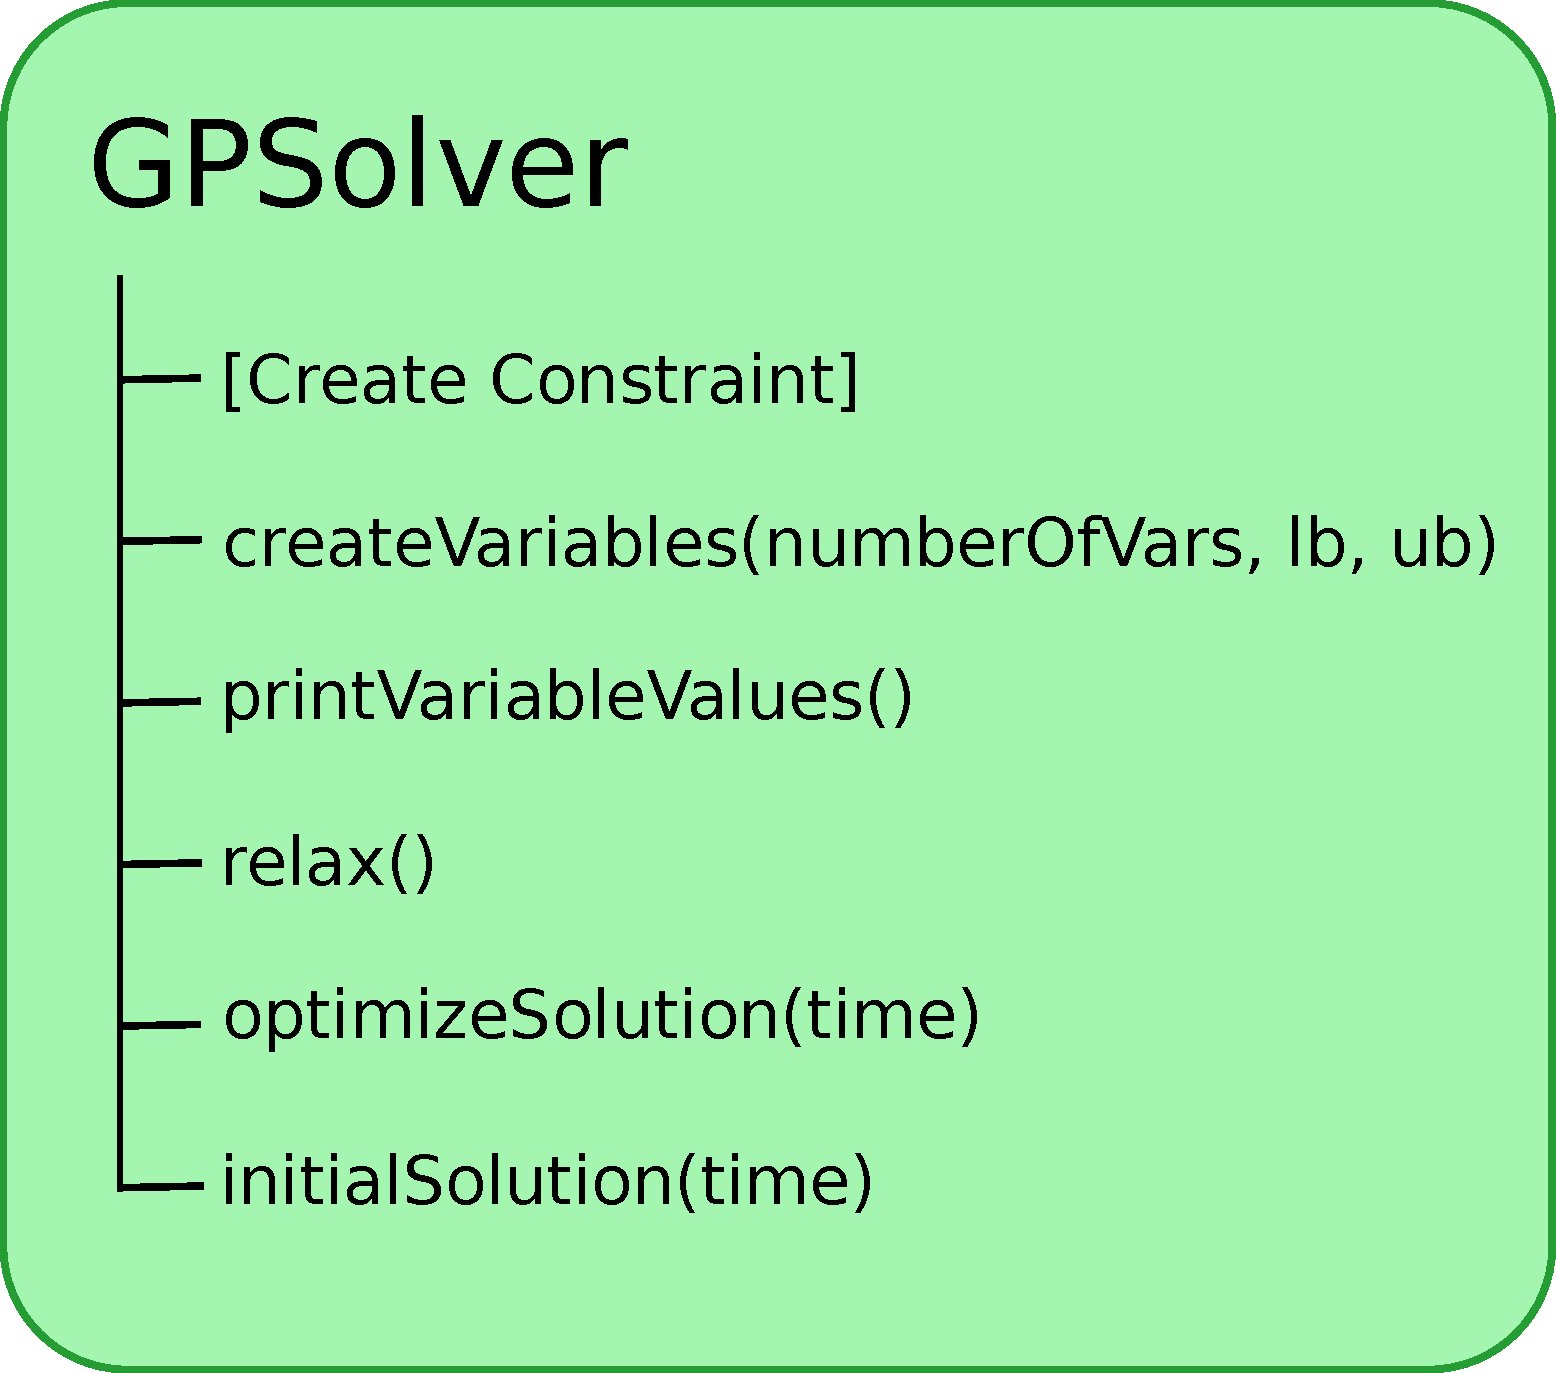
\includegraphics[width=0.8\linewidth]{general.pdf} \caption{Important methods in GPSolver class} 
\label{fig_general}
\end{center} 
\end{figure} 
The method \method{createVariables} takes three arguments to create a number of variables. The first argument 
is the number of variables to create with the given lower and upper bound, the second and third argument respectively. 
The method creates both the gecode variables used in the \class{GecodeEngine} and variables used in the 
\class{LocalSearchEngine} class. The variables used in the \class{LocalSearchEngine} class (LS variables) are of the 
class 
\class{Variable} and each has a pointer to the associated Gecode variable. The method returns pointers to the LS 
variables. \\ 
The method \method{relax} is only used if an initial solution could not be found within the limits given. It controls 
how the instance should be relaxed to find an initial solution. There is currently only one method implemented that 
relaxes the an instance that is described in subsection \ref{sub_inisol}. \\
All constraint available are created by calling the associated method in \gensol, that calls the constructor 
of the constraint and the method in \class{GecodeEngine} for posting the constraint in a Gecode space. The constraint 
objects should not be created directly by the user since the Gecode \class{Space} class is not available to the 
user. \\ 
To implements a new constraint object it must inheriting from the \class{Constraint} class 
and two methods, one in \class{GPSolver} and one in \class{GecodeEngine}, must be implemented. The method in 
\class{GecodeEngine} must post the constraint in the \class{GecodeEngine} space. The method in \class{GPSolver} 
should call the constructor of the constraint implemented and call the method in \class{GecodeEngine}. The solver must 
be able to reproduce the call to \class{GecodeEngine} in case it an initial solution is not found within the limits 
given. The relaxation method must be updated to handle the new constraint implemented as well. \\
To find an initial solution the method \method{initialSolution} must be called and it takes an integer argument. The 
argument indicates the time Gecode is allowed to search for an initial solution before \method{relax} is called. Once 
\method{relax} is called the same time limit is given again. \\
To find a better solution than the initial solution the method \method{optimizeSolution} can be called with a time 
limit as argument. That method starts the local search that is described in section \ref{sec_local}. 